% !TeX root = ../main.tex

\newlecture[Expectation][Sep 22, 2026]
\subsection{Expectation}

In STA237:
\[E(X) = \begin{cases*}
    \sum_{x}^{}x\cdot p(x) &\text{if } X \text{ discrete}\\
    \int xf(x)\,dx &\text{if } X \text{ continuous}
\end{cases*}\]
for this course, we are defining probability via ``measure theory'', so we need to revisit the definition of expectation.

Particularly, under the ``measure theory'' perspective:
\[E(X) = \int x\, dP \quad \Rightarrow P = \text{probability measure}\]
\[\int xf(x)\,dx \quad \Rightarrow \quad \int x\, dP\]
``Riemann Integral'' \aside{(integrating against a measure $dP$ instead of $dx$; this is the Lebesgue integral)}

\begin{definition}[Simple Expectation][5.1]
    If $X$ only takes finitely many values $x_1, \dots, x_n$, and $A_i = \left\{\omega: X(\omega) = x_i\right\}$, define the expectation of $X$ by:
    \[E(X) = \sum_{i=1}^{n}x_i P(A_i)\]
\end{definition}

\begin{example}[][5.1.1]
    For an arbitrary set $A \subset \Omega$, let
    \[Y(\omega) = I\left\{\omega \in A\right\} \qquad \text{Then } E(Y) = P(A)\]
    \begin{align*}
        E(Y) &= \sum_{i=0}^{1}y_i \cdot P(A_i) \qquad Y\text{ only takes two values 0 and 1}\\
        &= 1 \cdot P\left\{\omega \in A\right\} + 0\cdot P\left\{\omega \notin A\right\}\\
        &= P(A) = P(\left\{\omega: \omega \in A\right\})
    \end{align*}
\end{example}


\begin{example}[][5.1.2]
    $P$ is uniform measure on $\Omega = [0,1)$, and
    \[X(\omega) = \begin{cases}
        5 & \omega > \frac{1}{3} \\
        3 & \omega \leq \frac{1}{3}
    \end{cases}\]
    \begin{center}
    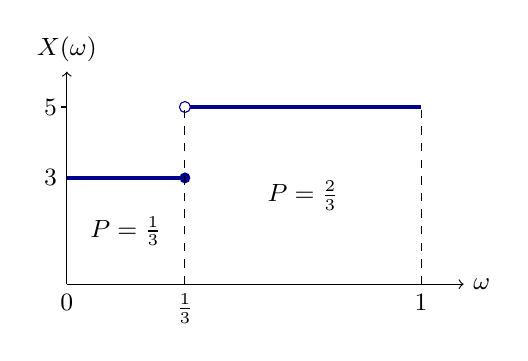
\begin{tikzpicture}[xscale=4.5, yscale=0.45, every node/.style={font=\small}]
        \draw[->] (0,0) -- (1.12,0) node[right]{$\omega$};
        \draw[->] (0,0) -- (0,6) node[above]{$X(\omega)$};
        \draw[very thick, blue!55!black] (0,3) -- (1/3,3);
        \draw[very thick, blue!55!black] (1/3,5) -- (1,5);
        \node[circle, fill=blue!55!black, inner sep=1.4pt] at (1/3,3) {};
        \node[circle, draw=blue!55!black, fill=white, inner sep=1.4pt] at (1/3,5) {};
        \draw[dashed] (1/3,0) -- (1/3,5);
        \draw[dashed] (1,0) -- (1,5);
        \node[below] at (0,0) {$0$};
        \node[below] at (1/3,0) {$\frac{1}{3}$};
        \node[below] at (1,0) {$1$};
        \node[left] at (0,3) {$3$};
        \node[left] at (0,5) {$5$};
        \draw (0,5) -- (-0.015,5);
        \node at (1/6,1.5) {\aside{$P = \frac13$}};
        \node at (2/3,2.5) {\aside{$P = \frac23$}};
    \end{tikzpicture}
    \end{center}
    \[E(X) = 5 \cdot P(\omega > \frac{1}{3}) + 3\cdot P(\omega \leq \frac{1}{3})\]
    \[=5\cdot (1-\frac{1}{3}) + 3\cdot \frac{1}{3}\]
    \[ = \frac{13}{3}\]
\end{example}

\begin{proposition}[Properties of Expectation][5.2]
    If $X$ and $Y$ are simple random variables, the following hold:
    \begin{enumerate}[label = \roman*)]
        \item If $X\geq 0$ a.s., $E(X) \geq 0$
        \item For any $a \in \mathbb{R}$, $E(aX) = a \cdot E(X)$
        \item $E(X+Y) = E(X)+E(Y)$
    \end{enumerate}
    Remark: "a.s." means almost surely.
    if $E$ a.s. $\Rightarrow$ $P(E) = 1$
    \\  $X \geq 0$ a.s. $\Rightarrow$ $P(X \geq 0) = 1$ $\Leftrightarrow$ $P(\left\{\omega: X(\omega) \geq 0\right\})=1$
    \\we may have certain $\omega$'s s.t. $X(\omega) < 0$, but $P(\left\{\omega: X(\omega) < 0\right\}) = 0$
\end{proposition}

Proof: Both i) and ii) are trivial.
\\For iii), let $X$ take values $x_1, \dots, x_n$ on sets $A_1,\dots, A_n$ (i.e. $A_i = \left\{\omega: X(\omega) = x_i\right\}$) and $Y$ takes values $y_1, \dots, y_m$ on sets $B_1, \dots, B_m$.
\\Observe that there are $m\cdot n$ events
\[C_{ij} = \left\{X = x_i \bigcap Y = y_j \right\}\]
Then
\begin{align*}
    E(X+Y) &= \sum_{i=1}^{n}\sum_{j=1}^{m} (x_i+y_j)\cdot P(C_{ij})\\
    &= \sum_{i=1}^{n}x_i \sum_{j=1}^{m} P(X=x_i \cap Y=y_j)+\sum_{j=1}^{m}y_j \sum_{i=1}^{n} P(X=x_i \cap Y=y_j)\\
    &= \sum_{i=1}^{n}x_i P(X=x_i)+\sum_{j=1}^{m}y_j P(Y=y_j)\\
    &= E(X)+E(Y)
\end{align*}
\hfill $\square$

\begin{lemma}[][5.2.1]
    If Proposition 5.2 holds, the following properties also hold:
    \begin{enumerate}[label = \roman*), start=4]
        \item If $X \leq Y$ a.s., then $E(X) \leq E(Y)$
        \item If $X=Y$ a.s., then $E(X) = E(Y)$
        \item $\left|E(X)\right| \leq E(\left|X\right|)$
    \end{enumerate}
    proof as exercise.
\end{lemma}

Our logic is, we first define
\begin{center}
    expectation of simple random variables
    \\$\Downarrow$
    \\expectation of bounded R.V.'s (approximation)
    \\$\Downarrow$
    \\expectation of non-negative R.V's (truncation)
    \\$\Downarrow$
    \\expectation of any R.V.'s (symmetric)
\end{center}

\begin{definition}[Bounded Random Variable][5.3]
    A random variable $X$ is bounded if there exists
    $M< \infty$, such that $|X|\leq M$ a.s.
\end{definition}

\begin{definition}[Expectation of Bounded Random Variable][5.3.1]
    If $X$ is a bounded R.V., then
    \begin{align*}
        E(X) &= \inf\left\{ E(Z): Z \text{ simple, }Z \geq X \text{ a.s.}\right\}\\
        &= \sup\left\{E(Y): Y \text{ simple, }Y \leq X \text{ a.s.}\right\}
    \end{align*}
\end{definition}

Recall, when we defined the integral:
\\the integral is defined as the limit value of sums of areas of tiny rectangles.
\begin{center}
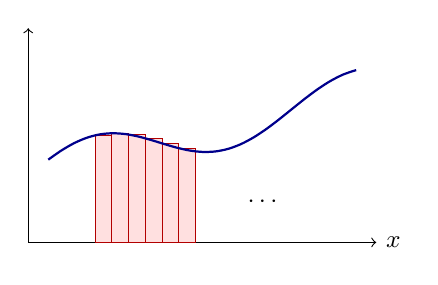
\begin{tikzpicture}[scale=0.85, every node/.style={font=\small}]
    \draw[->] (0,0) -- (5.2,0) node[right]{$x$};
    \draw[->] (0,0) -- (0,3.2);
    \foreach \x in {1.0,1.25,...,2.25} {
        \pgfmathsetmacro{\h}{0.35*sin(deg(1.6*\x))+0.25*\x+1.0}
        \draw[red!70!black, fill=red!12] (\x,0) rectangle (\x+0.25,\h);
    }
    \draw[thick, blue!55!black, domain=0.3:4.9, smooth, variable=\x] plot ({\x}, {0.35*sin(deg(1.6*\x))+0.25*\x+1.0});
    \node at (3.5,0.6) {$\cdots$};
\end{tikzpicture}
\end{center}
When it comes to the Riemann integral, we are no longer cutting $X$ axis into tiny intervals, but cutting each set into tiny subsets and calculate the sum of $x$ times the measure of each tiny subset.
\begin{align*}
    E(X) &= \inf \left\{E(Z): \quad Z\text{ is simple and } Z \geq X \text{ a.s.}\right\}\\
    &= \sup \left\{E(Y): \quad Y \text{ is simple and } Y \leq X \text{ a.s.}\right\}
\end{align*}
\begin{center}
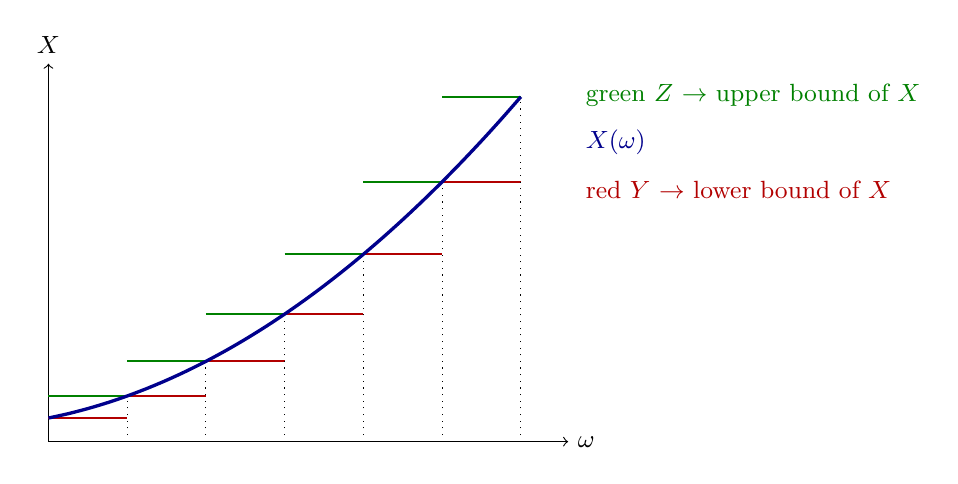
\begin{tikzpicture}[scale=1, every node/.style={font=\small}]
    \draw[->] (0,0) -- (6.6,0) node[right]{$\omega$};
    \draw[->] (0,0) -- (0,4.8) node[above]{$X$};
    \foreach \a in {0,1,...,5} {
        \pgfmathsetmacro{\lo}{0.08*\a*\a+0.2*\a+0.3}
        \pgfmathsetmacro{\hi}{0.08*(\a+1)*(\a+1)+0.2*(\a+1)+0.3}
        \draw[thick, green!50!black] (\a,\hi) -- (\a+1,\hi);
        \draw[thick, red!70!black] (\a,\lo) -- (\a+1,\lo);
        \draw[dotted] (\a+1,0) -- (\a+1,\hi);
    }
    \draw[very thick, blue!55!black, domain=0:6, smooth, variable=\x] plot ({\x}, {0.08*\x*\x+0.2*\x+0.3});
    \node[anchor=west, green!50!black] at (6.7,4.4) {green $Z$ $\to$ upper bound of $X$};
    \node[anchor=west, blue!55!black] at (6.7,3.8) {$X(\omega)$};
    \node[anchor=west, red!70!black] at (6.7,3.2) {red $Y$ $\to$ lower bound of $X$};
\end{tikzpicture}
\end{center}
``Squeeze the R.V. $X$ via two simple R.V.'s $Y$ and $Z$, with one capturing the upper bound and the other capturing the lower bound''.
\\Proof: Since $X$ is bounded, $|X| < M$ a.s.
\[L = \sup \left\{EY: \quad Y \text{ simple and }Y\leq X \text{ a.s.}\right\}\]
\[U = \inf\left\{EZ: \quad Z \text{ simple and }Z \geq X \text{ a.s.}\right\}\]
\[L \leq U \text{ as } Y\leq X \text{ a.s. and }Z\geq X \text{ a.s.}\]
Our goal is to prove $L \geq U \quad \Rightarrow \quad L = U \overset{def}{=}E(X)$
\\the way to cut $[-M, M]$ into tiny intervals.
\\for any arbitrary $n$, we define
\[E_k = \left\{\omega: \frac{kM}{n}\geq X(\omega) \geq \frac{(k-1)M}{n}\right\}\]
\begin{center}
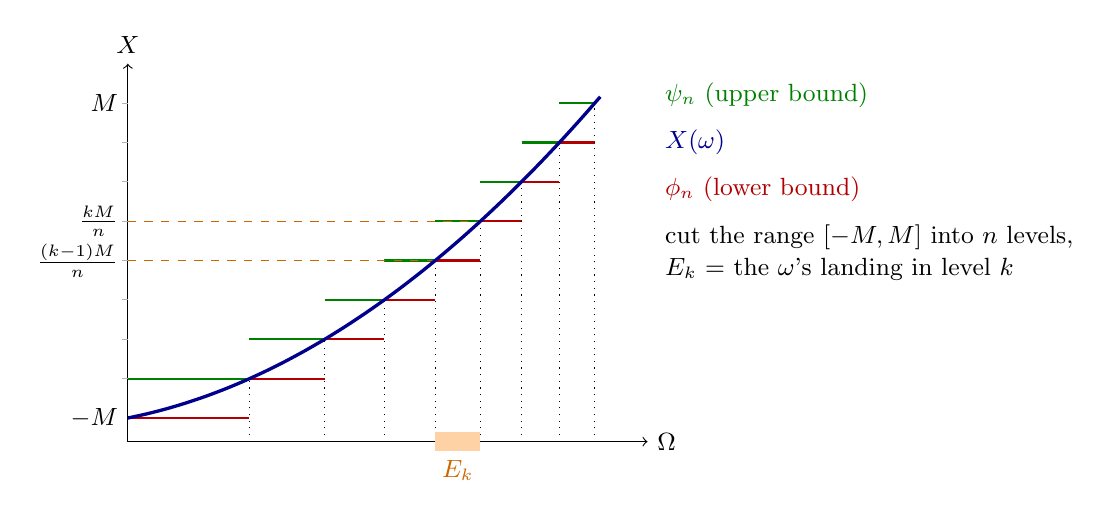
\begin{tikzpicture}[scale=1, every node/.style={font=\small}]
    % inverse of X(w) = 0.08 w^2 + 0.2 w + 0.3, to find where each level is hit
    \def\Xinv#1{(-0.2+sqrt(0.04+0.32*((#1)-0.3)))/0.16}
    \draw[->] (0,0) -- (6.6,0) node[right]{$\Omega$};
    \draw[->] (0,0) -- (0,4.8) node[above]{$X$};
    \foreach \k in {1,...,8} {
        \pgfmathsetmacro{\ylo}{0.5*\k-0.5+0.3}
        \pgfmathsetmacro{\yhi}{0.5*\k+0.3}
        \pgfmathsetmacro{\wlo}{max(0,\Xinv{\ylo})}
        \pgfmathsetmacro{\whi}{\Xinv{\yhi}}
        \draw[thick, green!50!black] (\wlo,\yhi) -- (\whi,\yhi);
        \draw[thick, red!70!black] (\wlo,\ylo) -- (\whi,\ylo);
        \draw[dotted] (\whi,0) -- (\whi,\yhi);
        \draw[gray!60] (-0.08,\yhi) -- (0,\yhi);
    }
    % highlight one E_k
    \pgfmathsetmacro{\wa}{\Xinv{2.3}}
    \pgfmathsetmacro{\wb}{\Xinv{2.8}}
    \fill[orange!35] (\wa,-0.12) rectangle (\wb,0.12);
    \node[below, orange!80!black] at ({(\wa+\wb)/2},-0.12) {$E_k$};
    \draw[dashed, orange!80!black] (0,2.3) -- (\wa,2.3);
    \draw[dashed, orange!80!black] (0,2.8) -- (\wb,2.8);
    \node[left] at (0,2.3) {$\frac{(k-1)M}{n}$};
    \node[left] at (0,2.8) {$\frac{kM}{n}$};
    \node[left] at (0,0.3) {$-M$};
    \node[left] at (0,4.3) {$M$};
    \draw[very thick, blue!55!black, domain=0:6, smooth, variable=\x] plot ({\x}, {0.08*\x*\x+0.2*\x+0.3});
    \node[anchor=west, green!50!black] at (6.7,4.4) {$\psi_n$ (upper bound)};
    \node[anchor=west, blue!55!black] at (6.7,3.8) {$X(\omega)$};
    \node[anchor=west, red!70!black] at (6.7,3.2) {$\phi_n$ (lower bound)};
    \node[anchor=west] at (6.7,2.4) {\aside{\shortstack[l]{cut the range $[-M,M]$ into $n$ levels,\\ $E_k$ = the $\omega$'s landing in level $k$}}};
\end{tikzpicture}
\end{center}

we then define two simple R.V.'s
\\Lower bound: \[\phi_n(\omega) = \sum_{k}^{}\frac{(k-1)M}{n}\cdot I(\omega \in E_k)\]
\\Upper bound: \[\psi_n(\omega) = \sum_{k}^{}\frac{kM}{n}\cdot I(\omega \in E_k) \]
\[\phi_n(\omega) \leq X(\omega) \leq \psi_n(\omega)\]
\[E\phi_n(\omega) \leq E(X) \leq E\psi_n(\omega)\]
\[E\psi_n(\omega) = E\phi_n(\omega) + \frac{M}{n}\]
Let $n\to\infty$, \quad $\dfrac{M}{n} \to 0$, so the upper bound and lower bound converge:
\[L \geq E\phi_n = E\psi_n - \frac{M}{n} \geq U - \frac{M}{n} \quad \Rightarrow \quad L \geq U\]
\[E(X) = E\psi_n(\omega) = E\phi_n(\omega) \quad \text{as } n\to\infty\]
\hfill $\square$

$X \leq Y$ a.s. means:
\begin{enumerate}[label = step \arabic*.]
    \item $\omega: X(\omega) \leq Y(\omega)$
    \item $\left\{ \omega: X(\omega) \leq Y(\omega)\right\}$
    \item $P(\left\{ \omega: X(\omega) \leq Y(\omega)\right\}) = 1$
\end{enumerate}
then we say $X \leq Y$ a.s.

\begin{definition}[Non-negative Random Variable][5.4]
    If $X \geq 0$ a.s. ($P(\left\{\omega: X(\omega)\geq 0\right\}) = 1$)
    \\define $E(X) = \sup \left\{E(Y): Y\text{ bounded, } 0\leq Y \leq X \text{ a.s.}\right\}$
\end{definition}

\begin{center}
\begin{tikzpicture}[scale=1, every node/.style={font=\small}]
    \draw[->] (0,0) -- (6,0) node[right]{$\Omega$};
    \draw[->] (0,0) -- (0,4.5) node[above]{$X$};
    \draw[very thick, blue!55!black, domain=0.8:5.1, smooth, variable=\x] plot ({\x}, {0.6+0.5*sin(deg(\x-0.8))+0.012*(\x)^4});
    \draw[thick, red!70!black, domain=0.8:4.75, smooth, variable=\x] plot ({\x}, {min(3.2, 0.45+0.5*sin(deg(\x-0.8))+0.012*(\x)^4)});
    \draw[thick, red!70!black] (4.75,3.2) -- (5.1,3.2);
    \draw[dashed, red!70!black] (0,3.2) -- (4.75,3.2);
    \node[left, red!70!black] at (0,3.2) {bound};
    \node[anchor=west, blue!55!black] at (6.3,3.6) {$X$};
    \node[anchor=west, red!70!black] at (6.3,3.0) {$Y$: bounded, $0 \leq Y \leq X$ a.s.};
    \node[anchor=west, red!70!black] at (6.3,2.2) {$\sup\{E(Y)\} \to E(X)$};
\end{tikzpicture}
\end{center}

Remark: Def 5.4. only provides a definition of $E(X)$ when $X$ is non-negative, it does \underline{not} guarantee $E(X) < \infty$.

\begin{definition}[Integrable Random Variables][5.5]
    For any random variable $X$, let $X^+(\omega) = \max\left\{X(\omega), 0\right\}$, and $X^-(\omega) = \max\left\{-X(\omega), 0\right\}$.
    \\Observe that both $X^+$ and $X^-$ are non-negative and $X=X^+ - X^-$.
    \\Then, if $E(|X|) = E(X^+) + E(X^-) < \infty$, we say R.V. $X$ is integrable and define $E(X) = E(X^+) - E(X^-)$
\end{definition}

\begin{center}
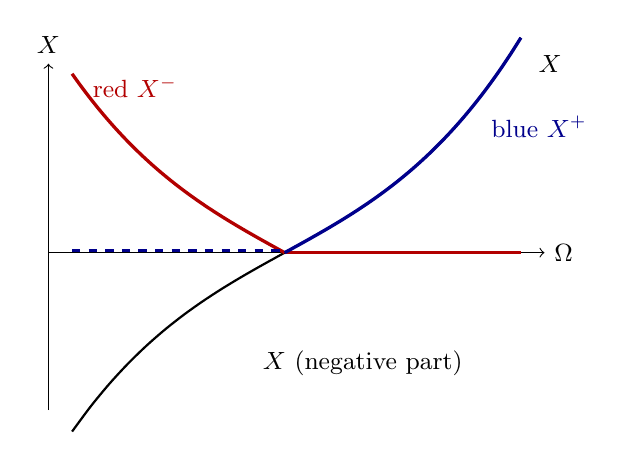
\begin{tikzpicture}[scale=1, every node/.style={font=\small}]
    \draw[->] (0,0) -- (6.3,0) node[right]{$\Omega$};
    \draw[->] (0,-2) -- (0,2.4) node[above]{$X$};
    \draw[thick, black, domain=0.3:6, smooth, variable=\x] plot ({\x}, {0.55*(\x-3)+0.04*(\x-3)*(\x-3)*(\x-3)});
    \draw[very thick, red!70!black, domain=0.3:3, smooth, variable=\x] plot ({\x}, {-0.55*(\x-3)-0.04*(\x-3)*(\x-3)*(\x-3)});
    \draw[very thick, red!70!black] (3,0) -- (6,0);
    \draw[very thick, blue!55!black, domain=3:6, smooth, variable=\x] plot ({\x}, {0.55*(\x-3)+0.04*(\x-3)*(\x-3)*(\x-3)});
    \draw[very thick, blue!55!black, dashed] (0.3,0.03) -- (3,0.03);
    \node[anchor=west] at (6.1,2.4) {$X$};
    \node[blue!55!black, anchor=west] at (5.5,1.6) {blue $X^+$};
    \node[red!70!black] at (1.1,2.1) {red $X^-$};
    \node[anchor=west] at (2.6,-1.4) {$X$ (negative part)};
\end{tikzpicture}
\end{center}

\begin{enumerate}
    \item $E|X| = E(X^+)+E(X^-) < \infty \Rightarrow X \text{ is integrable}$
    \item $E(X) = E(X^+) - E(X^-)$
\end{enumerate}

\begin{proposition}[Properties of Expected Values][5.6]
    If R.V. $X$ is either bounded, non-negative or integrable, Proposition 5.2 holds.
\end{proposition}
\begin{enumerate}
    \item $X$ and $Y$ may not need to be simple, if they are bounded, non-negative or integrable, the 3 properties (prop 5.2) also hold.
    \item Lemma 5.2.1 says, if prop 5.2 holds, the additional 3 properties also hold.
    \item To sum up, if R.V.'s are bounded, non-negative or integrable, all the 6 properties hold.
\end{enumerate}

Hint for Assignment 1. Q2:
\begin{quote}
    $E_1$ and $E_2$ are independent.
    \\$E_1^c$ and $E_2^c$ are independent.

    if $E_1, E_2, \dots E_n$, you want to prove $E_1^c, E_2^c, \dots E_n^c$ are independent.
    \[P(E_1^c \bigcap E_2^c \bigcap \cdots \bigcap E_n^c) = \cdots\]
    you can flip 1 event at a time

    first try to flip the first\dots
    \[P(E_1^c \bigcap E_2 \bigcap E_3 \bigcap \cdots \bigcap E_n)\]
    \[= P(E_2 \bigcap E_3 \bigcap \cdots \bigcap E_n) - P(E_1 \bigcap E_2 \bigcap \cdots \bigcap E_n)\]
    \[ = \cdots = (1-P(E_1))P(E_2)\cdots P(E_n)\]

    Then you flip the second one\dots
    \[P(E_1^c \bigcap E_2^c \bigcap E_3 \bigcap \cdots \bigcap E_n)\]
    Via induction, complete the proofs
\end{quote}
